%
%===============>>  Ленотьева Модуль 7 <<=============
%
\setmodule{8}

%BEGIN_FOLD % ====>>_____ Занятие 1 _____<<====
\begin{class}[number=1]
	\begin{listofex}
		\item 
		\begin{minipage}[t]{\bodywidth}
			На клетчатой бумаге с размером клетки 1х1 изображён параллелограмм. Найдите его площадь.
		\end{minipage}
		\hspace{0.02\linewidth}
		\begin{minipage}[t]{\picwidth}
			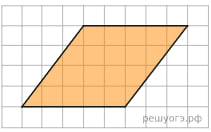
\includegraphics[align=t, width=\linewidth]{../../../../../exercises/lists/pics/leontevaM8L1-1}
		\end{minipage}
		\item 
		\begin{minipage}[t]{\bodywidth}
			На клетчатой бумаге с размером клетки 1х1 изображён параллелограмм. Найдите его площадь.
		\end{minipage}
		\hspace{0.02\linewidth}
		\begin{minipage}[t]{\picwidth}
			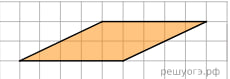
\includegraphics[align=t, width=\linewidth]{../../../../../exercises/lists/pics/leontevaM8L1-2}
		\end{minipage}
		\item Найдите величину острого угла параллелограмма \( ABCD \), если биссектриса угла \( A \) образует со стороной \( BC \) угол, равный \( 43\degree \). Ответ дайте в градусах.
		\item В параллелограмме \( ABCD \) диагональ \( AC \) в \( 2 \) раза больше стороны \( AB \) и \( \angle ACD=111\degree \). Найдите угол между диагоналями параллелограмма. Ответ дайте в градусах.
		\item Диагональ \( BD \)  параллелограмма \( ABCD \)  образует с его сторонами углы, равные \( 50\degree \) и \( 85\degree \). Найдите уголы параллелограмма.
		\item В прямоугольнике диагональ равна \( 10 \), а угол между ней и одной из сторон равен \( 60\degree \), длина этой стороны равна \( 5 \). Найдите площадь прямоугольника, деленную на \( \sqrt{3} \).
		\item В прямоугольнике одна сторона равна \( 96 \), а диагональ равна \( 100 \). Найдите площадь прямоугольника.
		\item Найдите площадь квадрата, если его диагональ равна \( 3 \).
		\item Найдите площадь прямоугольника, если его периметр равен \( 102 \), а отношение соседних сторон равно \(  2:15 \).
		\item На экзамене \( 25 \) билетов, Сергей не выучил \( 3 \) из них. Найдите вероятность того, что ему попадётся выученный билет.
		\item Коля выбирает трехзначное число. Найдите вероятность того, что оно делится на \( 5 \).
		\item Телевизор у Маши сломался и показывает только один случайный канал. Маша включает телевизор. В это время по трем каналам из двадцати показывают кинокомедии. Найдите вероятность того, что Маша попадет на канал, где комедия не идет.
		\item На тарелке \( 12 \) пирожков: \( 5 \) с мясом, \( 4 \) с капустой и \( 3 \) с вишней. Наташа наугад выбирает один пирожок. Найдите вероятность того, что он окажется с вишней.
		\item В каждой десятой банке кофе согласно условиям акции есть приз. Призы распределены по банкам случайно. Варя покупает банку кофе в надежде выиграть приз. Найдите вероятность того, что Варя не найдет приз в своей банке.
		\item В случайном эксперименте симметричную монету бросают дважды. Найдите вероятность того, что орел выпадет ровно \( 1 \) раз.
		\item Игральную кость бросают дважды. Найдите вероятность того, что оба раза выпало число, большее \( 3 \).
		
	\end{listofex}
\end{class}
%END_FOLD

%BEGIN_FOLD % ====>>_____ Занятие 2 _____<<====
\begin{class}[number=2]
	\begin{listofex}
		
		\item Решите уравнение \( x^{2} =2x+8 \).
		\item Найдите корень уравнения \( (x + 10)(- x - 8)=0 \).
		\item Решите уравнение  \( -x^{2}-6x+16=0 \). Если корней больше одного, в ответе укажите бóльший корень.
		\item Решите уравнение: \( \dfrac{5x}{9}=\dfrac{1}{8}:\mfrac{3}{3}{4} \)
		\item 
		\begin{minipage}[t]{\bodywidth}
			На клетчатой бумаге нарисованы два круга. Площадь внутреннего круга равна 15 м. Найдите площадь заштрихованной фигуры. 
		\end{minipage}
		\hspace{0.02\linewidth}
		\begin{minipage}[t]{\picwidth}
			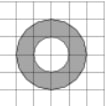
\includegraphics[align=t, width=\linewidth]{../../../../../exercises/lists/pics/leontevaM8L2-3}
		\end{minipage}
		\item \( AC \) и \( BD \)  — диаметры окружности с центром \( O \). Угол \( ACB \) равен \( 55\degree \). Найдите угол \( AOD \). Ответ дайте в градусах.
		\item Центр окружности, описанной около треугольника \( ABC \), лежит на стороне \( AB \). Найдите угол \( ABC \), если угол \( BAC \) равен \( 74\degree \). Ответ дайте в градусах.
		\item Отрезок \( AB  =  8 \) касается окружности радиуса \( 6 \) с центром \( O \) в точке \( B \). Окружность пересекает отрезок \( AO \) в точке \(  D \). Найдите \( AD \).
		\item На окружности по разные стороны от диаметра \( AB \) взяты точки \( M \) и \( N \). Известно, что \( \angle NBA  =  38\degree \). Найдите угол \( NMB \). Ответ дайте в градусах.
		
		
	\end{listofex}
\end{class}
%END_FOLD

%BEGIN_FOLD % ====>>_ Домашняя работа 1 _<<====
\begin{homework}[number=1]
	\begin{listofex}
		\item Вычислите:
		\begin{tasks}(2)
			\task \( \dfrac{6,9-1,5}{2,4} \)
			\task \( \dfrac{2,4}{2,9-1,4} \)
			\task \( \dfrac{9,4}{4,1+5,3} \)
			\task \( \dfrac{6,9+4,1}{0,2} \)
		\end{tasks}
		\item В случайном эксперименте симметричную монету бросают четыре раза. Найдите вероятность того, что орел выпадет ровно \( 2 \) раза.
		\item 
		\begin{minipage}[t]{\bodywidth}
			Найдите площадь параллелограмма, изображенного на рисунке.
		\end{minipage}
		\hspace{0.02\linewidth}
		\begin{minipage}[t]{\picwidth}
			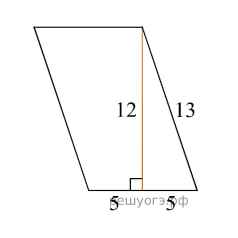
\includegraphics[align=t, width=\linewidth]{../../../../../exercises/lists/pics/leontevaM8L2-1}
		\end{minipage}
		\item В параллелограмме \( ABCD \) диагональ \( AC \) в \( 2 \) раза больше стороны \( AB \) и \( \angle ACD=19\degree \). Найдите угол между диагоналями параллелограмма. Ответ дайте в градусах.
		\item В ромбе \( ABCD \) угол \( ABC \) равен \( 72\degree \). Найдите угол \( ACD \). Ответ дайте в градусах.
		\item Центральный угол \(  AOB \) опирается на хорду \( AB \) длиной \( 6 \). При этом угол \( OAB \) равен \( 60\degree \). Найдите радиус окружности.
		\item В окружности с центром в точке \( О \) проведены диаметры \( AD \) и \( BC \), угол \( OCD \) равен \( 30\degree \). Найдите величину угла \( OAB \).
	\end{listofex}
\end{homework}
%END_FOLD

%BEGIN_FOLD % ====>>_____ Занятие 3 _____<<====
\begin{class}[number=3]
	\begin{listofex}
		\item 
		\begin{minipage}[t]{\bodywidth}
			Дано \( \angle 1 = \angle 2 \), \( \angle 2=140\degree \). Найти \( \angle 4 \).
		\end{minipage}
		\hspace{0.02\linewidth}
		\begin{minipage}[t]{\picwidth}
			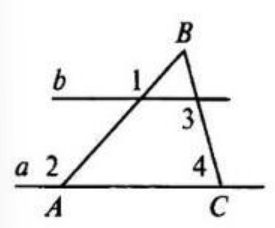
\includegraphics[align=t, width=\linewidth]{../../../../../exercises/lists/pics/leontevaM7L3-3}
		\end{minipage}
		\begin{minipage}[t]{\bodywidth}
			\item Дано: \( a || b \), \( c \) – секущая, \( \angle 1 - \angle 2 = 102\degree \).Найти все образовавшиеся углы.
		\end{minipage}
		\hspace{0.02\linewidth}
		\begin{minipage}[t]{\picwidth}
			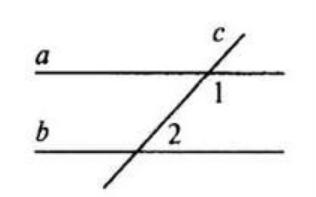
\includegraphics[align=t, width=\linewidth]{../../../../../exercises/lists/pics/leontevaM7L3-2}
		\end{minipage}
		\item Отрезок \( AD \) - биссектриса треугольника \( ABC \). Через точку \( D \) проведена прямая, параллельная стороне \( AB \) и пересекающая сторону \( AC \) в точке \( F \).
		Найти углы треугольника \( ADF \), если \( \angle BAC=72\degree \).
		\item 
		\begin{minipage}[t]{\bodywidth}
			При перемечении двух параллельных прямых секущей образованно 8 углов. Угол 1 равен \( 150\degree \). Найдите остальные углы.
		\end{minipage}
		\hspace{0.02\linewidth}
		\begin{minipage}[t]{\picwidth}
			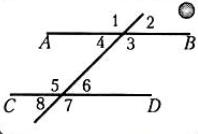
\includegraphics[align=t, width=\linewidth]{../../../../../exercises/lists/pics/leontevaM7L3-1}
		\end{minipage}
		\item В мешке содержатся жетоны с номерами от \( 5 \) до \( 54 \) включительно. Какова вероятность, того, что извлеченный наугад из мешка жетон содержит двузначное число?
		\item Игральную кость бросают дважды. Найдите вероятность того, что сумма двух выпавших чисел равна \( 4 \) или \( 7 \).
		\item Определите вероятность того, что при бросании игрального кубика (правильной кости) выпадет нечетное число очков.
		\item Касательные в точках \( A \) и \( B \) к окружности с центром в точке \( O  \) пересекаются под углом \( 82\degree \). Найдите угол \( ABO \). Ответ дайте в градусах.
		\item Отрезки \( AB \) и \( CD \) являются хордами окружности. Найдите длину хорды \( CD \), если \( AB  =  30 \), а расстояния от центра окружности до хорд \( AB \) и \( CD \) равны соответственно \( 20 \) и \( 15 \).
		\item Найдите площадь кругового сектора, если градусная мера его дуги равна 30º, а радиус круга равен 6 см.
		\item Радиус круга равен \( 3 \), а длина ограничивающей его окружности равна \( 6\pi \). Найдите площадь круга. В ответ запишите площадь, деленную на \( \pi \).
		\item Радиус круга равен \( 1 \). Найдите его площадь, деленную на \( \pi \).
		\item Боковая сторона равнобедренного треугольника равна 4. Угол при вершине, противолежащий основанию, равен \( 120\degree \). Найдите диаметр окружности, описанной около этого треугольника.
		\item Радиус окружности, описанной около квадрата, равен \( 16\sqrt{2} \). Найдите длину стороны этого квадрата.
		
	\end{listofex}
\end{class}
%END_FOLD

%BEGIN_FOLD % ====>>_____ Занятие 4 _____<<====
\begin{class}[number=4]
	\begin{listofex}
		\item  На одном из рисунков изображен график функции \( y=x^{2}-2x +3 \). Укажите номер этого рисунка.
		\begin{figure}[h!]
			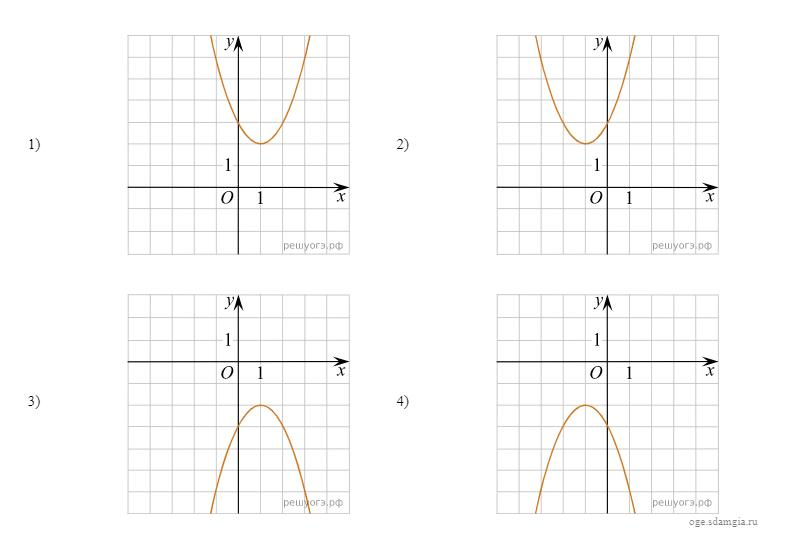
\includegraphics[align=t, width=\linewidth]{../../../../../exercises/lists/pics/leontevaM8L4-1}
		\end{figure}
		\newpage
		\item Установите соответствие между функциями и их графиками.	
		\begin{tasks}(1)
			\task \( y=x^{2}- 2x \)
			\task \( y=x^{2}+ 2x \)
			\task \( y=-x^{2}- 2x \)
		\end{tasks}
		\begin{figure}[h!]
			\caption{}
			\label{fig:leontevam8l4-2}
			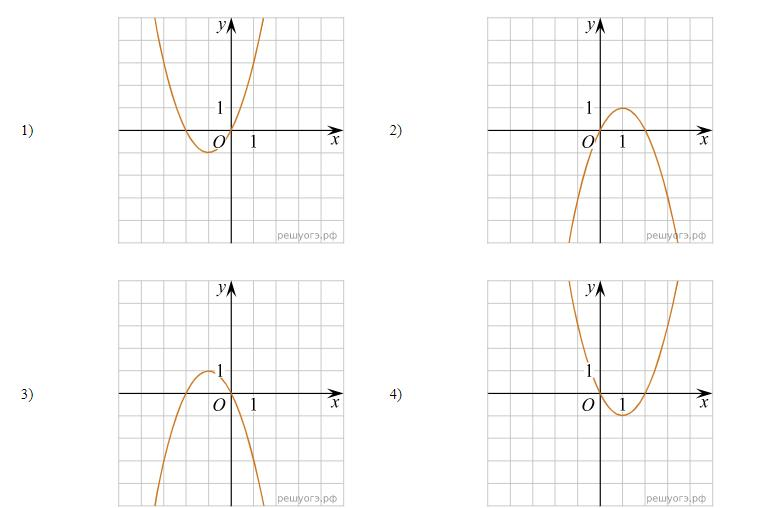
\includegraphics[align=t, width=\linewidth]{../../../../../exercises/lists/pics/leontevaM8L4-2}
		\end{figure}
		\newpage
		\item На рисунке изображены графики функций вида y  =  ax2 + c. Установите соответствие между графиками и знаками коэффициентов a и c.
		\begin{tasks}(1)
			\task  \( a > 0 \), \( c < 0 \)	
			\task  \( a < 0 \), \( c > 0 \)	
			\task \( a > 0 \), \( c > 0 \)	
			\task \( a < 0 \), \( c < 0 \)
		\end{tasks}
		\begin{figure}[h!]
			\caption{}
			\label{fig:leontevam8l4-3}
			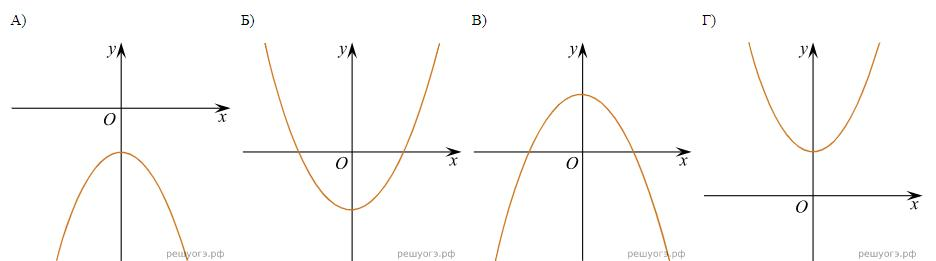
\includegraphics[align=t, width=\linewidth]{../../../../../exercises/lists/pics/leontevaM8L4-3}
		\end{figure}
		\item В прямоугольнике одна сторона равна \( 96 \), а диагональ равна \( 100 \). Найдите площадь прямоугольника.
		\item 
		\begin{minipage}[t]{\bodywidth}
			На клетчатой бумаге с размером клетки \( 1x1 \) изображён ромб. Найдите длину его большей диагонали.
		\end{minipage}
		\hspace{0.02\linewidth}
		\begin{minipage}[t]{\picwidth}
			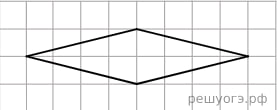
\includegraphics[align=t, width=\linewidth]{../../../../../exercises/lists/pics/leontevaM8L2-2}
		\end{minipage}
		\item 
		\begin{minipage}[t]{\bodywidth}
			На клетчатой бумаге с размером клетки \( 1 \)см \( x \) \( 1 \)см изображён параллелограмм. Найдите длину его большей высоты. Ответ дайте в сантиметрах.
		\end{minipage}
		\hspace{0.02\linewidth}
		\begin{minipage}[t]{\picwidth}
			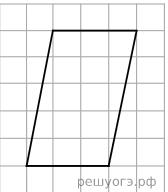
\includegraphics[align=t, width=\linewidth]{../../../../../exercises/lists/pics/leontevaM8L4-4}
		\end{minipage} 
		\item Диагонали \( AC \) и \( BD \) параллелограмма \( ABCD \) пересекаются в точке \( O \), \( AC  =  14 \), \( BD  =  18 \), \( AB  =  5 \). Найдите\(  DO \).
		\item Найдите острый угол параллелограмма \( ABCD \), если биссектриса угла \( A \) образует со стороной \( BC \) угол, равный \( 41\degree \). Ответ дайте в градусах.
		\item В параллелограмме \( ABCD \) диагональ \( AC \) в \( 2 \) раза больше стороны \( AB \) и \( \angle ACD=19\degree \). Найдите угол между диагоналями параллелограмма. Ответ дайте в градусах.
		\item В ромбе \( ABCD \) угол \( ABC \) равен \( 72\degree \). Найдите угол \( ACD \). Ответ дайте в градусах.
		\item Площадь ромба равна \( 63 \), а периметр равен \( 36 \). Найдите высоту ромба.
		\item На стороне \( BC \) прямоугольника \( ABCD \), у которого \( AB = 48 \) и \( AD = 112 \), отмечена точка \(  E \) так, что \( \angle EAB = 45\degree \). Найдите \( ED \).
		\item В угол \( C \) величиной \( 88\degree \) вписана окружность, которая касается сторон угла в точках \( A \) и \( B \), точка \( O \) – центр окружности. Найдите угол \( AOB \). Ответ дайте в градусах.
		\item Касательные в точках \( A \) и \( B \) к окружности с центром \( O \) пересекаются под углом \( 66\degree \). Найдите угол \( ABO \). Ответ дайте в градусах.
	\end{listofex}
\end{class}
%END_FOLD

%BEGIN_FOLD % ====>>_ Домашняя работа 2 _<<====
\begin{homework}[number=2]
	\begin{listofex}
		\item 
		\begin{minipage}[t]{\bodywidth}
			Дано: \( AB || CD \), \( AB = BC \), \( \angle ABF = 45\degree \). Найти: \( \angle ACD \).
		\end{minipage}
		\hspace{0.02\linewidth}
		\begin{minipage}[t]{\picwidth}
			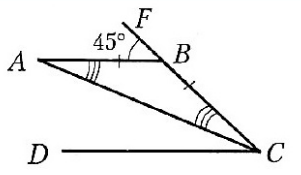
\includegraphics[align=t, width=\linewidth]{../../../../../exercises/lists/pics/leontevaM8H2-1}
		\end{minipage}
		\item Дано: треугольники \( ABC = DEF \), \( AC \) и \( DF \) лежат на одной прямой. Доказать: 1) \( BC || EF \), 2) \( AB || DE \).
		\item Вероятность того, что новая шариковая ручка пишет плохо (или не пишет), равна 0,19. Покупатель в магазине выбирает одну такую ручку. Найдите вероятность того, что эта ручка пишет хорошо.
		\item Стрелок 4 раза стреляет по мишеням. Вероятность попадания в мишень при одном выстреле равна 0,5. Найдите вероятность того, что стрелок первые 3 раза попал в мишени, а последний раз промахнулся.
		\item  Радиус вписанной в квадрат окружности равен \( 2\sqrt{2}  \). Найдите радиус окружности, описанной около этого квадрата.
		\item Центральный угол \( AOB \) опирается на хорду \( AB \) длиной 6. При этом угол \( OAB \) равен \( 60\degree \). Найдите радиус окружности.
	\end{listofex}
\end{homework}
%END_FOLD

%BEGIN_FOLD % ====>>_____ Занятие 5 _____<<====
\begin{class}[number=5]
	\begin{listofex}
		\item Занятие 5
	\end{listofex}
\end{class}
%END_FOLD

%BEGIN_FOLD % ====>>_____ Занятие 6 _____<<====
\begin{class}[number=6]
	\begin{listofex}
			\item Пробник
	\end{listofex}
\end{class}
%END_FOLD

%BEGIN_FOLD % ====>>_ Домашняя работа 3 _<<====
\begin{homework}[number=3]
	\begin{listofex}
		\item Найдите значение выражения \( \dfrac{11}{5}-1,6+\dfrac{13}{4}\cdot\mfrac{3}{24}{45}-\dfrac{3}{23}\cdot1,34 \).
		\item Какому из данных промежутков принадлежит число   \( \dfrac{5}{9} \)? 
		\begin{tasks}(4)
			\task \( [0,5;0,6] \)
			\task \( [0,6;0,7] \)
			\task \( [0,7;0,8] \)
			\task \( [0,8;0,9] \)
		\end{tasks}
		\item В треугольнике \( ABC \) угол \( C \) прямой, \( AC  =  8 \) , \( \cos A  = 0,4 \). Найдите \( AB \).
		\item В треугольнике \( ABC \) угол \( C \) равен \( 90\degree \), \( AC = 6 \), \( AB = 10 \). Найдите \( \sin B \).
		\item В треугольнике \( ABC \) угол \( C \) равен \( 90\degree \), \( BC = 14 \), \( AB = 50 \). Найдите \( \cos B. \)
		\item Камень бросают в глубокое ущелье. При этом в первую секунду он пролетает 9 метров, а в каждую следующую секунду на 10 метров больше, чем в предыдущую, до тех пор, пока не достигнет дна ущелья. Сколько метров пролетит камень за первые пять секунд?
		\item В амфитеатре 13 рядов. В первом ряду 17 мест, а в каждом следующем на 2 места больше, чем в предыдущем. Сколько всего мест в амфитеатре?
		\item Радиус окружности, описанной около квадрата, равен \( 44\sqrt{2} \). Найдите радиус окружности, вписанной в этот квадрат.
		\item Высота \( BH \) параллелограмма \( ABCD \) делит его сторону \( AD \) на отрезки \( AH  =  8 \) и \( HD  =  28 \). Диагональ параллелограмма \( BD \) равна 35. Найдите площадь параллелограмма.
		\item
			График какой из приведенных ниже функций изображен на рисунке?
		\begin{figure}[h]
			
		\center{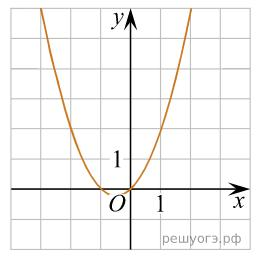
\includegraphics[align=t, width=0.2\linewidth]{../../../../../exercises/lists/pics/leontevaM8H3-1}}
		\end{figure}
		\begin{tasks}(4)
			\task \( y=x^{2}-x \)
			\task \( y=-x^{2}-x \)
			\task \( y=x^{2}+x \)
			\task \( y=-x^{2}+x \)
		\end{tasks}
	\newpage
		\item Решите неравенство:
		\begin{tasks}(2)
			\task \( (x-3)(5x-4)(8-x)\geq 0 \)
			\task \( x^{2}+3x+2\leq 0 \)
			\task \( x(x+10)(x-3)\geq 0 \)
			\task \( (4-x)(2x-5)<0 \)
			\task \( (x+7)^{10}(x-9)(x-8)^{5}\geq 0 \)
			\task \( (x+7)^{9}(x+8)(x-4)^{6}\geq 0 \)
		\end{tasks}
	\end{listofex}
\end{homework}
%END_FOLD

%BEGIN_FOLD % ====>>_____ Занятие 7 _____<<====
\begin{class}[number=7]
	\begin{listofex}
		\item[] На рисунке точками показано количество минут исходящих вызовов и трафик мобильного интернета в гигабайтах, израсходованных абонентом в процессе пользования смартфоном, за каждый месяц 2019 года. Для удобства точки, соответствующие минутам и гигабайтам, соединены сплошными и пунктирными линиями соответственно.
		\\\ \begin{figure}[h]
		\center{
			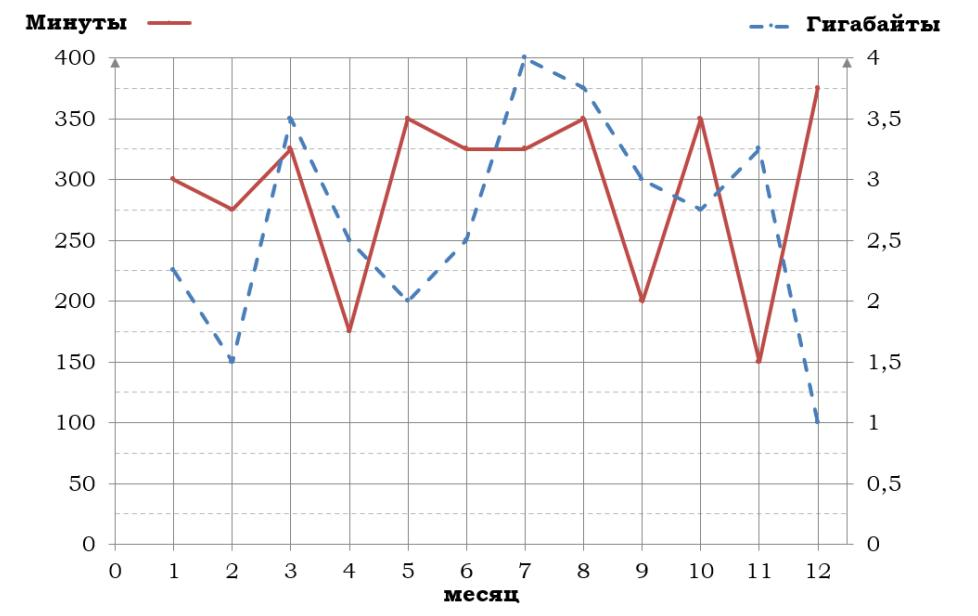
\includegraphics[align=t, width=\linewidth]{../../../../../exercises/lists/pics/leontevaM8L7-1}}
		\end{figure}\\\
		В течение года абонент пользовался тарифом «Стандартный», абонентская плата по которому составляла 360 рублей в месяц. При условии нахождения абонента на территории РФ в абонентскую плату тарифа «Стандартный» входит:
		\begin{itemize}
			\item пакет минут, включающий 300 минут исходящих вызовов на номера, зарегистрированные на территории РФ;
			\item пакет интернета, включающий 3 гигабайта мобильного интернета;
			\item пакет SMS, включающий 140 SMS в месяц;
			\item безлимитные бесплатные входящие вызовы.
		\end{itemize}
		Стоимость минут, интернета и SMS сверх пакета тарифа указана в таблице.
		\newpage
		\begin{figure}[h]
			\center{
				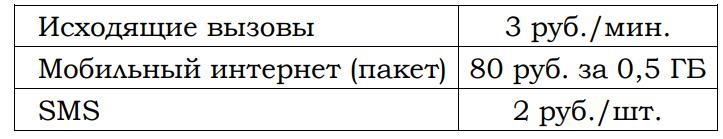
\includegraphics[align=t, width=0.5\linewidth]{../../../../../exercises/lists/pics/leontevaM8L7-2}}
		\end{figure}
		Абонент не пользовался услугами связи в роуминге. За весь год абонент отправил 125 SMS.
		\item Определите, какие месяцы соответствуют указанному в таблице трафику мобильного интернета. Заполните таблицу, в бланк ответов перенесите числа, соответствующие номерам месяцев, без пробелов, запятых и других дополнительных символов.
		\begin{figure}[h]
			\center{
				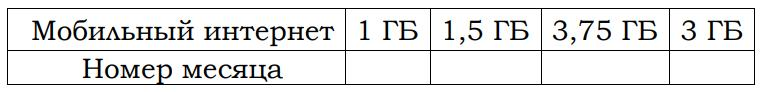
\includegraphics[align=t, width=0.5\linewidth]{../../../../../exercises/lists/pics/leontevaM8L7-3}}
		\end{figure}
		\item Сколько рублей потратил абонент на услуги связи в феврале?
		
		\item Сколько месяцев в 2019 году абонент превысил лимит и по пакету минут, и по пакету мобильного интернета?
		\item Исходящие вызовы:
		\begin{tasks}(1)
			\task[A)]  Какое наибольшее количество минут исходящих вызовов за месяц было в 2019 году?
			\task[Б)] Какое наименьшее количество минут исходящих вызовов за месяц было в 2019 году? 
		\end{tasks}
		\item В конце 2019 года оператор связи предложил абоненту перейти на новый тариф, условия которого приведены в таблице.\\\
		\begin{figure}[h]
			\center{
				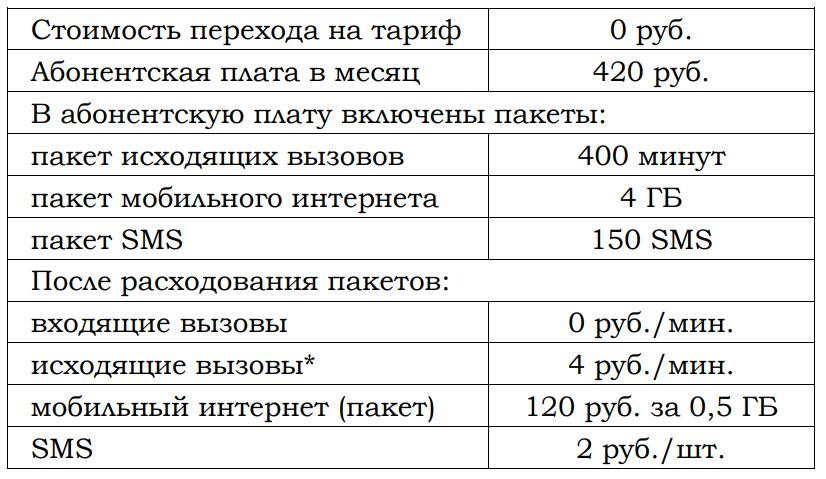
\includegraphics[align=t, width=0.5\linewidth]{../../../../../exercises/lists/pics/leontevaM8L7-6}}
		\end{figure}
		\\\ *исходящие вызовы на номера, зарегистрированные на территории РФ
		\\\ 
		\\\ Абонент решает, перейти ли ему на новый тариф, посчитав, сколько бы он потратил на услуги связи за 2019 г., если бы пользовался им. Если получится меньше, чем он потратил фактически за 2019 г., то абонент примет решение сменить тариф. 
		\\\ Перейдёт ли абонент на новый тариф? В ответе запишите ежемесячную абонентскую плату по тарифу, который выберет абонент на 2020 год.
			\end{listofex}
	
\begin{listofex}
	 	\item Определите, какие месяцы соответствуют указанному в таблице количеству исходящих вызов. Заполните таблицу, в бланк ответов перенесите числа, соответствующие номерам месяцев, без пробелов, запятых и других дополнительных символов.
		\begin{figure}[h]
			\center{
				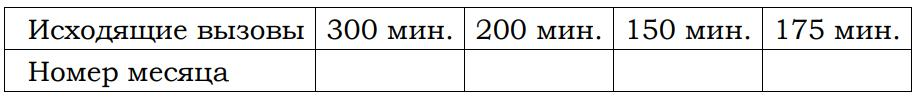
\includegraphics[align=t, width=0.5\linewidth]{../../../../../exercises/lists/pics/leontevaM8L7-4}}
		\end{figure}
		\item Сколько рублей потратил абонент на услуги связи в августе?
		\item На сколько процентов уменьшился трафик мобильного интернета в сентябре по сравнению с августом 2019 года?
		\item Пользуясь рисунком, поставьте в соответствие каждому из указанных периодов времени характеристику израсходованных минут и гигабайтов.
		\\\	\begin{figure}[h]
			\center{
				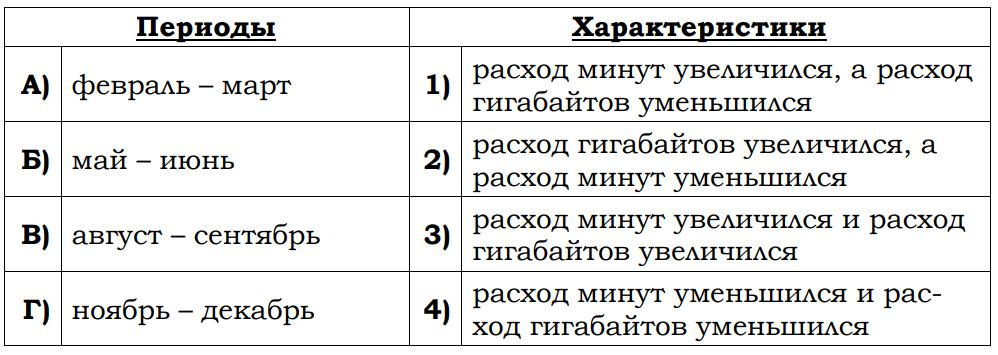
\includegraphics[align=t, width=0.7\linewidth]{../../../../../exercises/lists/pics/leontevaM8L7-5}}
		\end{figure}\\\
		В таблице под каждой буквой укажите соответствующий номер. В ответ запишите последовательность цифр без пробелов, запятых и других дополнительных символов.
	 
		 
		\item Абонент хочет приобрести новый смартфон. В трёх салонах сотовой связи этот смартфон продаётся в кредит (сначала делается первоначальный взнос, а потом ежемесячно в течение всего срока кредита вносятся платежи) на разных условиях. Условия приведены в таблице.\\\
		\begin{figure}[h]
			\center{
				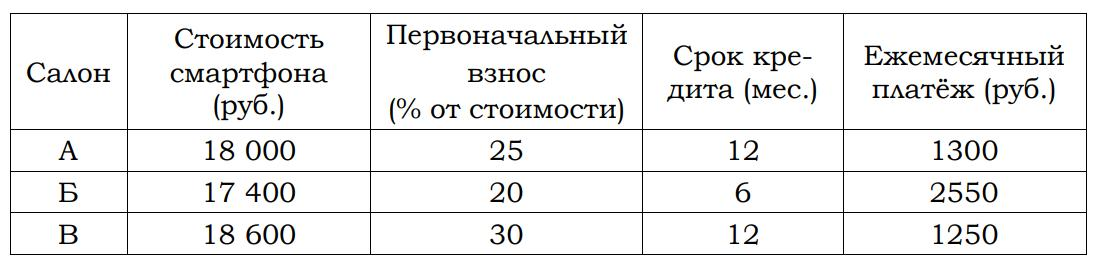
\includegraphics[align=t, width=0.6\linewidth]{../../../../../exercises/lists/pics/leontevaM8L7-7}}
		\end{figure}
		\\\ Определите, в каком из салонов покупка смартфона с учётом полностью выплаченного кредита обойдётся дешевле. В ответ запишите эту сумму в рублях.
		
		\item В амфитеатре 10 рядов. В первом ряду 25 мест, а в каждом следующем на 3 места больше, чем в предыдущем. Сколько мест в восьмом ряду амфитеатра?
		\item В ходе распада радиоактивного изотопа его масса уменьшается вдвое каждые 7 минут. В начальный момент масса изотопа составляла 640 мг. Найдите массу изотопа через 42 минуты. Ответ дайте в миллиграммах.
		\item В ходе биологического эксперимента в чашку Петри с питательной средой поместили колонию микроорганизмов массой 13мг. За каждые 30 минут масса колонии увеличивается в 3 раза. Найдите массу колонии микроорганизмов через 90 минут после начала эксперимента. Ответ дайте в миллиграммах.
	\end{listofex}
\end{class}
%END_FOLD

%BEGIN_FOLD % ====>>_ Проверочная работа _<<====
\begin{exam}
	\begin{listofex}
		 \item В 2020 году абонентская плата по тарифу «Стандартный» повысилась
		на \( 20\% \). Сколько рублей составила абонентская плата в 2020 году?
		
		\item Сколько рублей потратил абонент на услуги связи в августе? 
		\item Сколько месяцев в 2019 году абонент не превышал лимит по пакету исходящих минут? 
		\item Сколько месяцев в 2019 году абонент превысил лимит по пакету мобильного интернета?
		\item Сколько месяцев в 2019 году расходы по тарифу составили ровно 360 рублей?
		\item Трафик мобильного интернета:
		\begin{tasks}(1)
			\task[A)] Какой наибольший трафик мобильного интернета в гигабайтах за месяц
			был в 2019 году?
			\task[Б)] Какой наименьший трафик мобильного интернета в гигабайтах за месяц был в 2019 году?
		\end{tasks}
		\item На сколько процентов увеличилось количество минут исходящих вызовов в октябре по сравнению с сентябрём 2019 года?
		\item Известно, что в 2019 году абонентская плата по тарифу «Стандартный» снизилась на \( 10\% \) по сравнению с 2018 годом. Сколько рублей составляла абонентская плата в 2018 году? 
		\item В январе 2020 года абонентская плата по тарифу «Стандартный» повысилась и составила 486 рублей. На сколько процентов повысилась абонентская плата?
	\end{listofex}
\end{exam}
%END_FOLD